%%%%%%%%%%%%%%%%%%%%%%%%%%%%%%%%%%%%%%%%%%%%%%%%%%%%%%%%%%%%%%%%%%%%%%%%%%%%%%%%%
%%%%%                             DATA SAMPLE                                %%%%
%%%%%%%%%%%%%%%%%%%%%%%%%%%%%%%%%%%%%%%%%%%%%%%%%%%%%%%%%%%%%%%%%%%%%%%%%%%%%%%%%

Our main data is a panel at the US postal service zipcode-month level from January 2010 to December 
2019. This panel comes from five distinct sources.

First of all, our data contains MW changes at the federal, state, county, and city level.\footnote{
	Note that federal level MW changes still could induce meaningful variation as it is binding in 
	some zipcodes and not in others, so that identification does not come only from time series 
	variation. However, the last federal MW increase was in 2009 so changes used in our estimates come 
	from state, county, and city level.} 
Most of these changes come from \textcite{VaghulZipperer2016} and \textcite{CegnizEtAl2019}, but 
we updated this data for the years 2017, 2018, and 2019. For each zipcode we assume that the prevailing 
MW at a given month is the maximum between the required by the federal, state, county, and city levels. 
We only use MW changes that are binding, so only changes that actually change the maximum. In our 
baseline panel, we use 5,301 MW changes at the zipcode-month level. These changes are constructed out 
of 166 state level changes and 229 county and city level changes.

% In our baseline estimates we exclude county and city level changes because they might have different 
% effects on rents and amenities. We include prominent MW changes at those levels in robustness checks, 
% and in specifications that allow explicitly for heterogeneous effects at the different jurisdiction 
% levels.

Second, we use rent and house value data from properties listed in Zillow \parencite{zillow} in our 
sample period. Zillow is the leader online real estate and rental platform in the U.S., hosting more 
than 110 million homes and 170 million unique monthly users in 
2019.\footnote{\href{https://www.zillowgroup.com/facts-figures/}
	{\texttt{https://www.zillowgroup.com/facts-figures/}} (accessed on October 23rd, 2020).}  
Zillow provides the median rental and listing price (both total and per square foot) at which homes 
were listed on the platform. Time series are provided for different house types, and for different 
geographic aggregation level.\footnote{\href{https://www.zillow.com/research/data/}
	{https://www.zillow.com/research/data/} provides more information on the data shared by Zillow. 
	The availability of different time series changed over time, so not all series used for the 
	analysis might be still available to download.} 
We choose to focus on USPS zipcode level monthly time series so to capture the local behavior of the 
housing market. Clearly, even within a single zipcode, there could be great heterogeneity in terms of 
house sizes and types, making it more difficult to assess the impact of local intervention. In an 
effort to minimize price variation coming from houses' characteristics, such as the number of bedrooms, 
we focus our main analysis on the single family, condominium and cooperative homes (SFCC) series. 
This is by far the series with the largest number of non-missing zipcode, as it covers the most 
common U.S. rental house types. In 2018, roughly a third of the nation's 47.2 million rental units 
were single-family homes, while another 43 percent was made up from buildings with 5 or more units 
\parencite{JCHS2020}. We then select -- for all our analysis -- \textit{per square foot} 
variables: this allows us to reduce confonding variation based on supply-side factors such as land 
availability. A limitation in the use of Zillow data comes from the fact that we cannot observe the 
underlying number of houses listed for rent in a given month. Changes in the Zillow inventory 
therefore introduce additional variation in the reported median rental price.

In \autoref{tab:desc_stats}, we compare descriptive statistics for our data and for representative 
US aggregates from the 2010 Census and the 5 years 2008 ACS. Columns 1 and 2 report data for the 
whole universe of US zipcodes and for the top 100 US metropolitan areas respectively. In column 3 
we show the complete set of Zillow data. Finally, in column 4 we restrict our sample by balancing 
the panel keeping fixed the number of zipcodes only using zipcodes that have complete SFCC rental 
data (baseline sample). Focusing on our preferred series, Zillow provides information on rents for 
4,604 unique zipcodes accounting for 11.8 percent of the US zipcodes and 46.7 percent of the 2015 US population. 
The average median household annual income for those zipcodes is \$64,289, 22.5 percent higher than 
the same figure for the average US zipcode, but it is slightly lower than the figure for the average 
zipcode in the top 100 metropolitan areas. Zipcodes in the baseline sample are more populous and 
slightly higher income than the average US zipcode. Zillow is a real estate company and as such it 
is present in more dynamic rental markets. Those markets have a higher share of urban population, a 
higher share of college students, and a higher share of house for rent that the average US zipcode. 
For these reasons, and given that we will show that our effects are driven by the lower income 
zipcodes in our sample, we interpret our estimates as a lower bound for the true average treatment 
effect.

To ensure that our data correctly captures the price evolution of the US rental market, we compare 
Zillow's median rental price with 5 Small Area Fair Market Rents (SAFMRs) series for houses with 
different number of bedrooms (0, 1, 2, 3, and 4 or more) coming from the US Department of Housing and 
Urban Development (\citeyear{hud}). SAFMRs are calculated for zipcodes within metropolitan areas at a 
yearly level, and generally equal the 40th percentile of the rent distribution for that 
zipcode.\footnote{For more information on how SAFMRs are calculated, see page 41641 of the 
	\href{https://www.huduser.gov/portal/datasets/fmr/fmr2018/FY2018-FMR-Preamble.pdf}
	{Federal Register/Vol. 82, No. 169}} 
The yearly time series correlation between Zillow SFCC and all of the SAMFRs series is consistently 
above 90 percent. Single family houses, as well as condos and cooperative houses, are fairly loose 
categories and are therefore expected to vary in terms of the number of bedrooms they might have. For 
this reason, in \autoref{fig:trend_zillow_safmrwgt} we compare the Zillow SFCC series with a weighted 
combination of the different SAMFRs series.\footnote{To compute the weighted SAMFR series we proceed 
	as follows. First, we compute the national yearly average for both the Zillow SFCC and the 5 
	SAFMR series. Then, for each of the latter we compute the U.S. share of single family, condo, 
	and cooperative houses with that number of bedrooms using the \textit{American Housing Survey} 
	(AHS). To ensure comparability, we only use the estimated count for rental houses in this step. 
	(Additionally, AHS data is available only for years 2011, 2013, 2015, 2017, and 2019. We therefore 
	fill missing years with previous year's share.) Finally, we weight SAFMR series using the 
	aforementioned shares.} 
The Zillow rent data is always higher in levels. Part of this difference is intuitively related to the 
fact that Zillow reports median rent prices while SAFMRs are based on the 40th percentile of the rent 
distribution. The two series however show similar trends, confirming that Zillow rental series indeed 
captures the dynamics of the U.S. rental prices.

% As for the information on house values, Zillow has data on 10875 unique zipcode that correspond to 
% \%27.7 of the zipcodes and to \%78.9 of the 2015 population. The average median household annual 
% income for those zipcodes in 2015 was \$69556, which is \%17 higher than the same figure for all 
% the US zipcodes

\begin{table}[h!]
    \caption{Descriptive statistics and comparison with representative zipcodes}
    \centering
    \label{tab:desc_stats}    
    
% Table created by stargazer v.5.2.2 by Marek Hlavac, Harvard University. E-mail: hlavac at fas.harvard.edu
% Date and time: Sun, Nov 08, 2020 - 3:45:47 PM
\begin{tabular}{@{\extracolsep{5pt}} ccccc} 
\\[-1.8ex]\hline 
\hline \\[-1.8ex] 
 & U.S. & Top 100 CBSA & Full Panel & Est. Panel \\ 
\hline \\[-1.8ex] 
Population (millions) (2010) & $311.18$ & $189.71$ & $110.17$ & $50.62$ \\ 
Population as share of U.S. & $1$ & $0.61$ & $0.35$ & $0.16$ \\ 
Housing Units (millions) (2010) & $132.83$ & $78.74$ & $46.72$ & $21.32$ \\ 
Housing Units as share of U.S. & $1$ & $0.59$ & $0.35$ & $0.16$ \\ 
Urban Share (2010) & $0.46$ & $0.75$ & $0.96$ & $0.97$ \\ 
College Share (2010) & $0.46$ & $0.75$ & $0.96$ & $0.97$ \\ 
African-American Share (2010) & $0.46$ & $0.75$ & $0.96$ & $0.97$ \\ 
Hispanic Share (2010) & $0.10$ & $0.14$ & $0.17$ & $0.19$ \\ 
Elder Share (2010) & $0.15$ & $0.13$ & $0.12$ & $0.11$ \\ 
Poor Share (2010) & $0.46$ & $0.75$ & $0.96$ & $0.97$ \\ 
Unemployed Share (2010) & $0.09$ & $0.09$ & $0.09$ & $0.09$ \\ 
Mean HH income (2010) & $52,492.56$ & $62,773.64$ & $65,475.16$ & $66,919.72$ \\ 
Rent House Share (2010) & $0.29$ & $0.35$ & $0.38$ & $0.38$ \\ 
Work in same county share (2010) & $0.70$ & $0.68$ & $0.76$ & $0.76$ \\ 
Unique zipcodes & $38,893$ & $14,583$ & $3,315$ & $1,305$ \\ 
Share of state events & $$ & $$ & $0.03$ & $0.03$ \\ 
Share of county events & $$ & $$ & $0.001$ & $0.001$ \\ 
Share of  localevents & $$ & $$ & $0.003$ & $0.0005$ \\ 
Mean SFCC psqft rent & $$ & $$ & $1.30$ & $1.27$ \\ 
Unique zipcodes SFCC psqft rent & $$ & $$ & $3,316$ & $1,143$ \\ 
\hline \\[-1.8ex] 
\end{tabular} 

   	\begin{minipage}{0.95\textwidth} \footnotesize
		\vspace{3mm} 
		\textit{Notes}: The table shows average values for the full sample (column 3), and the 
		restricted balanced samples, our baseline (column 4). In column 1 we report demographic 
		statistics for the universe of USPS zipcode we were able to map. In column 2 we report 
		demographic statistics for the top 100 CBSA. All demographic information comes from the 2010 
		Census and the 5-years 2008-2012 ACS.  
	\end{minipage}
\end{table}

\begin{figure}[!h]
    \centering
    \caption{National Time Series for Zillow and SAFMR data}
    \label{fig:trend_zillow_safmrwgt}
    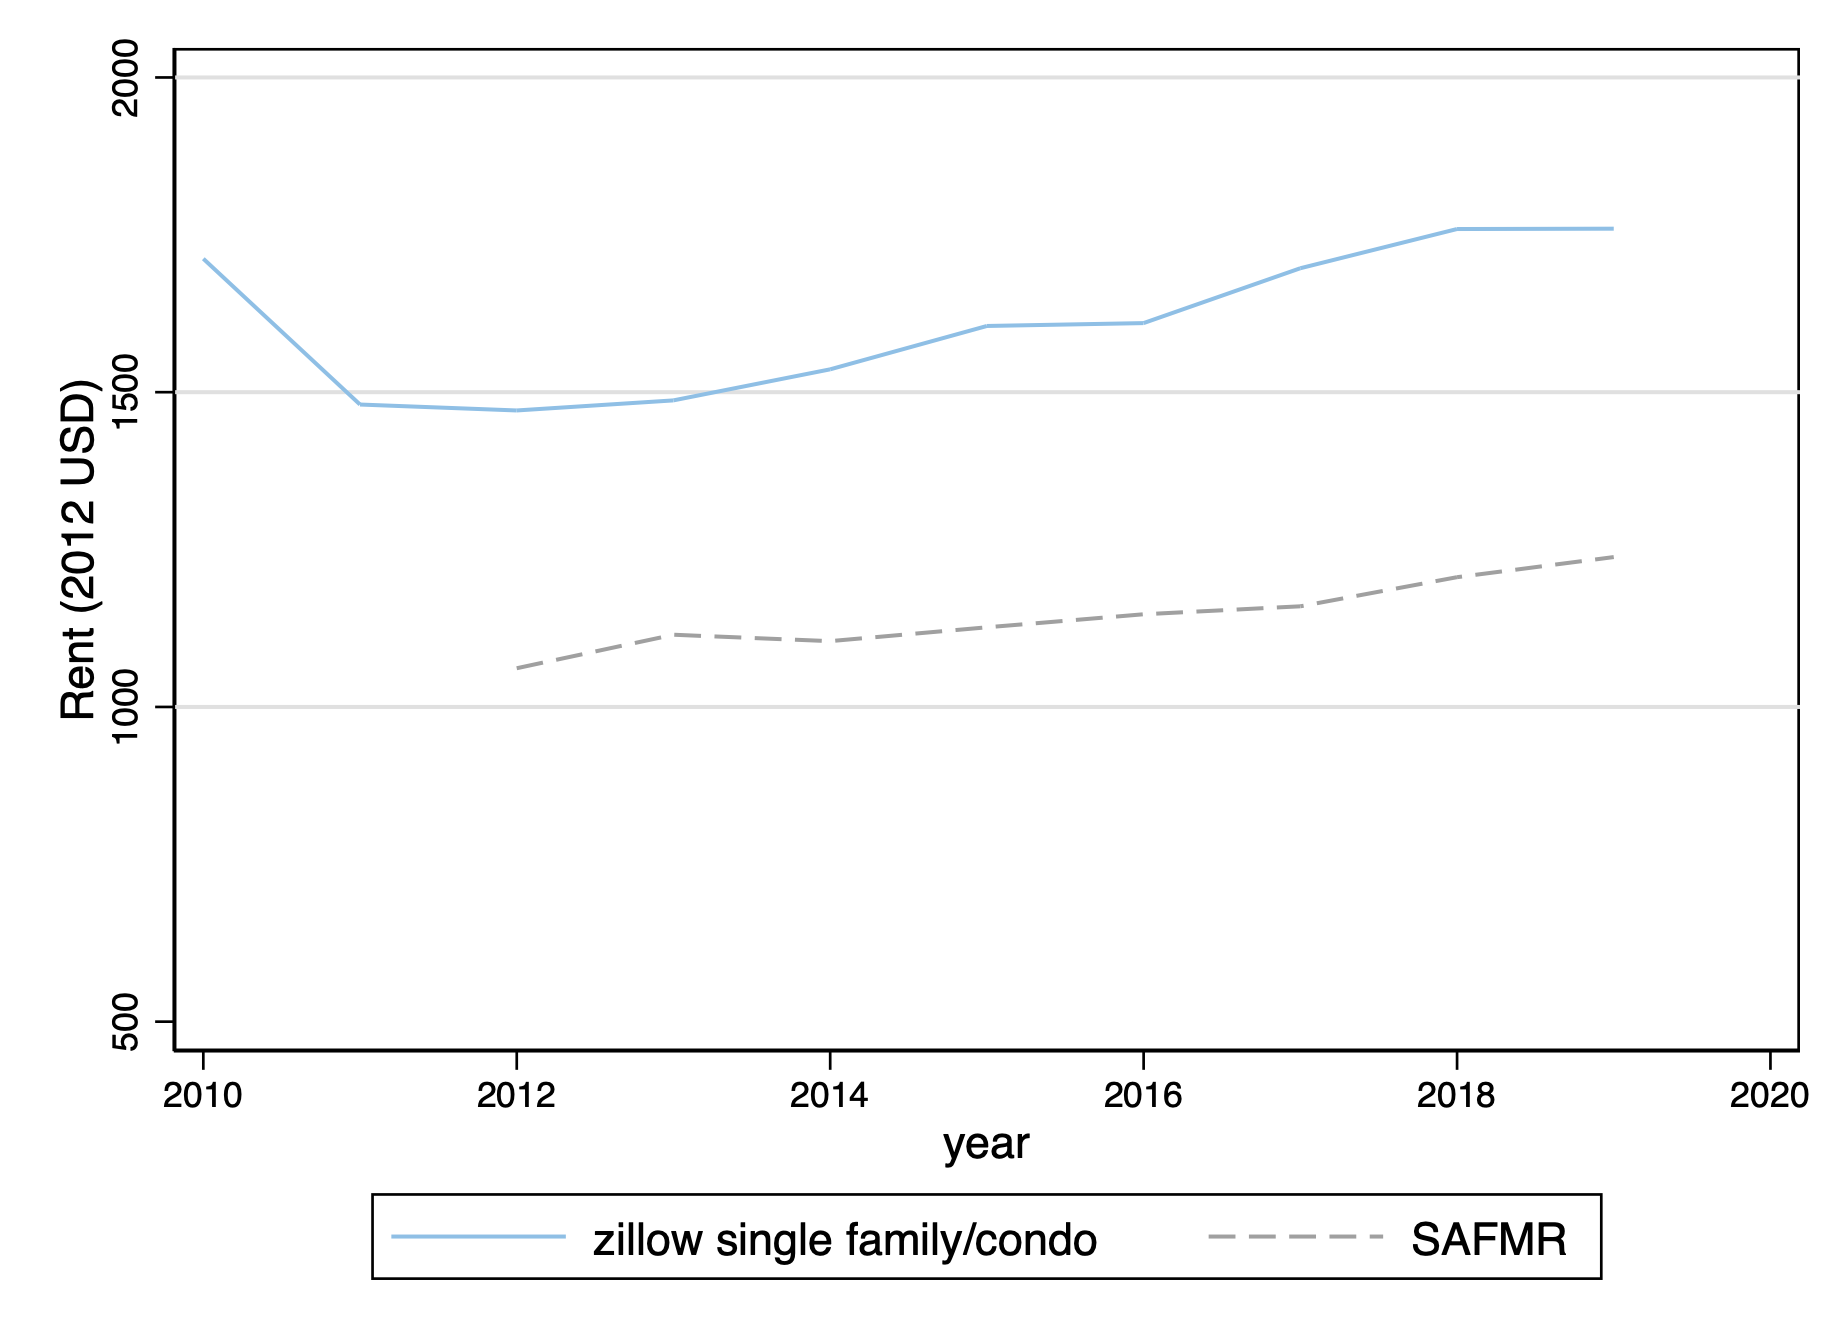
\includegraphics[width = 0.7\textwidth]{../../analysis/zillow_benchmark/output/trend_zillow_safmrwgt_zipcode_avg.png}
    \begin{minipage}{0.95\textwidth} \footnotesize
    	\vspace{3mm}
    	\textit{Notes:} The figure plots the monthly rent annual national average for the main Zillow 
    	series used in the analysis (SFCC) and a weighted combination of SAFMR series with different 
    	number of bedrooms. Weights are based on the US share of single family, condos and cooperative 
    	houses with given number of bedrooms as recorded in the AHS.    
    \end{minipage}
\end{figure}

Third, we add socio-demographic information to each zipcode in our sample using the 2010 Census and 
the 5-years 2008-2012 ACS. The data is originally obtained at the Census tract level and mapped into 
USPS zipcodes using HUD crosswalks.\footnote{Crosswalks are obtained from
	 \url{https://www.huduser.gov/portal/datasets/usps_crosswalk.html}} 
We assign to each zipcode the following characteristics: number of inhabitants, the number of houses, 
the median income, the number of black inhabitants, the number of unemployed, and the number of 
college students. We use this information to classify zipcodes into, for example, high or low median 
income to then perform heterogeneity analysis. In addition, given that zipcodes can cross county 
borders, we use the census data and geographic codes to map each zipcode to a county by assigning it 
to the one with the highest share of houses from that zipcode. We also map each zipcode to a 
metropolitan statistical area or a rural town analogously. We use this information to assign the 
prevailing MW to each zipcode.

% Fourth, to proxy for the quality of amenities at each location, we construct zipcode-month level 
% measures from GPS location point-of-interest data by SafeGraph\parencite{safegraph}. We define several 
% amenity measures. For our first measure, we follow closely \textcite{couture2019income} and construct 
% an index for the quality of restaurants available at each zipcode-month. This index is defined as the 
% average of the propensity of high-income individuals to visit a restaurant in a given zipcode 
% controlling for their distance to the establishments. In order to classify a visitor as high-income we 
% use the census tract location of the visitor. Our second measure is the same as the first but for the 
% quality of the visitors of open public spaces in each zipcode-month. For our third measure, we use the 
% point-of-interest data to count the number of restaurants, coffee shops, bars, and gyms per inhabitant 
% of a zipcode-month. 

Fourth, to proxy for local economic activity we collect data from the Quarterly Census of Employment 
and Wages (QCEW) at the county-quarter and county-month level for each industry and level of 
government.\footnote{The QCEW covers the following industries: goods-producing; natural resources and 
	mining; construction; manufacturing; service-providing; trade, transportation and utilities; 
	information; financial activities; professional and business services; education and health 
	services; leisure and hospitality. The QCEW additionally provides employment data for federal, 
	state, and local government.} 
For each county-quarter-industry cell we observe the number of establishments and the average weekly 
wage. For each county-month-industry cell we additionally observe the number of employed people. We 
merge this data onto our zipcode-month panel based on county and quarterly date.

We add data from the \textit{Building Permit Survey} (BPS) at the county-month level to account for 
time-varying shocks in the housing market. The BPS provides building permit statistics on new 
privately-owned residential construction disaggregated by house type. Lacking information on condos 
and cooperative houses, we only add the number of new units and the permits valuation for single 
family houses to each zipcode-month observation based on the county and month they belong.

Finally, we use data from the 2017 Longitudinal Employer-Household Dynamics Origin-Destination 
Employment Statistics (LODES) to proxy for MW workers' residence and workplace location. The LODES 
data sets provide block-level information on jobs and are organized in 3 groups: residence area 
characteristics (RAC), with information about characteristics of jobs for various types of workers 
(e.g. number of jobs in different sectors, number of job for workers under 30 years old, etc.); 
workplace area characteristics (WAC) that provide the same information as RAC files but aggregated 
with respect to workplace location; and a origin-destination matrix mapping jobs from residence to 
workplace locations. We use RAC and WAC datasets to ``locate" workers likely to be MW by looking at 
the state-level distribution of such type of workers: we build, for each zipcode in the sample, the 
share (out of the state total) of workers under 30 years old earning less than $\$1251$ that either 
\textit{live} or \textit{work} there. 
